\lohead{Hörmann Stefan}
\chapter{Mechanik}

\section{Anforderung}
\label{sec:Anforderung}
Die Arbeit des mechanischen Teiles besteht darin, eine Maschine,
die Spielkarten mischen und ausgeben kann zu entwerfen, zu konstruieren
und einen Teilaufbau durchzuführen. Die Maschine sollte in der Lage
sein 20 Spielkarten zu mischen und diese nach einem Spielmodus der
zuvor am LCD gewählt wurde auszugeben. Das Ziel ist es, die Spielkarten
optimal zu mischen, aber die Maschine dennoch kompakt und optisch
ansprechen zu entwerfen. Im weiteren sollte der Mischvorgang und die
Ausgabe der Karten nicht zu lange dauern. Die Teile der Maschine
sollten so konstruiert werden, dass sie kostengünstig produziert
werden können. Zum Schluss sollte noch ein Teilaufbau der Maschine
geschehen, um die Funktionalität der einzelnen Bereiche zu testen
und gegebenfalls zu verbessern.

\section{Problemstellungen}
Ein Problem ist das begrenzte Budget unseres Teams, somit sind
wir auf gewisse Produktionsarten unserer Bauteile beschränkt.
Dies hat zur Folge, dass die Bauteile oft sehr simpel sind um
sie leichter zu konstruieren. Die Oberfläche der Karten ist ein
weiteres Problem, da diese sich nicht immer separieren lassen, dies
verursacht, dass oft zwei oder mehrere Karten auf einmal genommen
werden und das Konzept des optimalen Mischens zerstört.

\section{Variantenvergleich}

\subsection{Anforderungen}

\begin{enumerate}
    \item \textbf{Kosten}  \\
    Der Automat sollte möglichst kostengünstig produziert werden,
    da das vorhandene Budget gering ist. Dies hat zur Folge das keine teuren Motoren
    oder ähnliche Bauteile zum Einsatz kommen können und keine teuren Bauteile produziert
    werden können.
    \item \textbf{Schnelligkeit} \\
    Um ein gutes Spielerlebnis zu garantieren, sollte der Automat keine
    langen Mischzeit besitzen. Die Dauer in der man die Karten einführt und auf den
    Mischen-Button klickt bis hin zur Ausgabe der ersten Karte sollte möglichst gering sein.
    \item \textbf{Mischgenauigkeit} \\
    Die Mischgenauigkeit ist die am schwersten gewichtete Anforderung,
    da es das Ziel ist ein optimales Mischen der Spielkarten zu erreichen, sollte
    diese Anforderung mit größter Wichtigkeit erfüllt werden.
    \item \textbf{Optik und Größe} \\
    Die Optik des Automaten soll schlicht gehalten werden, jedoch sollte
    sie dennoch auf Messen und andere Ausstellungen präsentierbar sein. Der Automat
    sollte jedoch auch stabil konstruiert werden, muss aber dennoch mobil bleiben und
    darf eine gewisse Größe nicht Überschreiten.
\end{enumerate}

\subsection{Variantenvergleich}
Um alle oben angegebenen Anforderungen zu erfüllen, wurden mehrere Konzepte entworfen und diese verglichen.

\subsubsection{Variante 1 - Linearachsen}

\begin{wrapfigure}{r}{0.6\textwidth}
    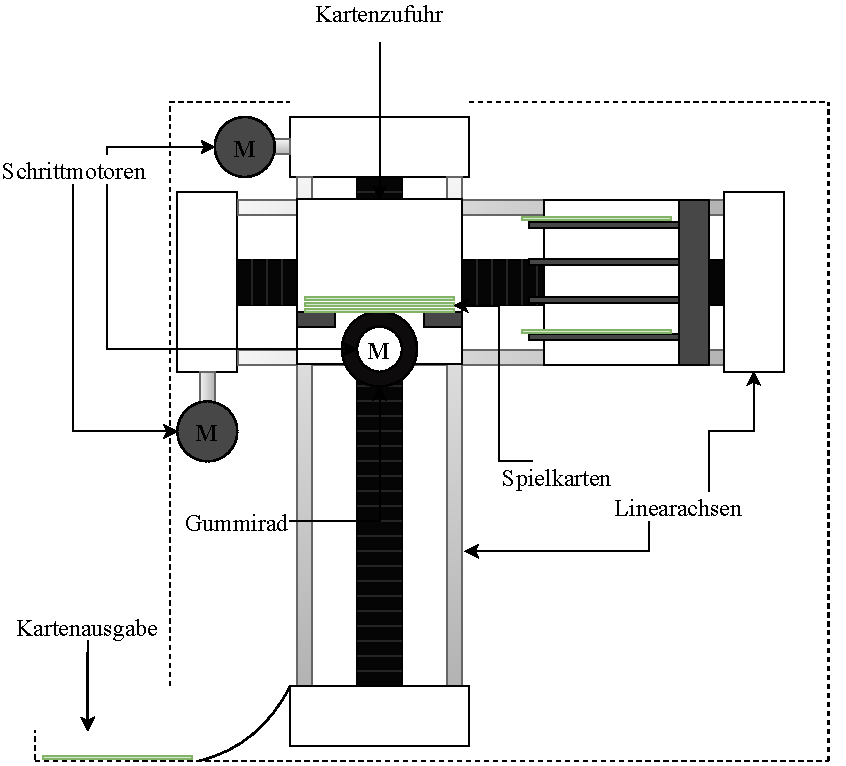
\includegraphics[width=0.6\textwidth]{fig/mech/Version1.pdf}
    \caption{Konzept 1}
\end{wrapfigure}

Das erste Konzept würde mit zwei Linearachsen realisiert werden, diese wären im rechten Winkel zueinander
angeordnet. Die Senkrechte Linearachse ist mit einer Halterung versehen, diese Halterung ist in der Lage
ein Kartendeck aufzunehmen und die unterste Karte mithilfe eines Ausgaberades weiterzubefördern. Die zweite
Linearachse besitzt 4 Fächer in der die Karten von der ersten Linearachsenausgabe zufällig befördert werden.
Dies wird realisiert indem die erste Linearachse bei jeder Ausgabe zufällig das Fach durch hinauf und
hinabfahren wechselt. Befinden sich alle Karten im Lager, so fährt die erste Linearachse nach unten, danach
fährt die zweite Linearachse impulsiv nach links, um die Karten aus dem Lager zu befördern. Diese fallen
Senkrecht in das Lager der ersten Linearachse, wo sie nun zum Ausgeben durch das Ausgaberad bereit liegen. \\



Durch die schnelle Bewegung der Linearachsen ist es möglich einen schnellen Mischprozess zu erreichen,
auch die Tatsache das es nur ein rotierendes Rad gibt und zwei Bewegliche Linearachsen führt dazu, das
Fehler bei Bewegungen nur selten Auftreten. Jedoch besteht durch den hohen Aufbau der Maschine und durch die hohe
Position der zweiten Linearachse die sich horizontal bewegt die Gefahr des umkippens der Maschine, und somit ist
keine stabilität mehr gegeben. Der Preis der Linearachsen ist ein weiterer Nachteil dieses Konzeptes, eine Linearachse
die unsere Anforderungen entspricht, wäre mit Motor und Schlitten zu teuer für unser Budget. \\

\textbf{Vorteile:}
\begin{itemize}
    \item schnelles Mischen
    \item wenige Fehlerquellen
\end{itemize}
\textbf{Nachteile:}
\begin{itemize}
    \item teuer
    \item großer Aufbau %Genaueres Beschreiben der Vor und Nachteile?
    \item instabil
\end{itemize}

\subsubsection{Variante 2 - Lagerrad mit Asugaberäder}

\begin{wrapfigure}{r}{0.6\textwidth}
    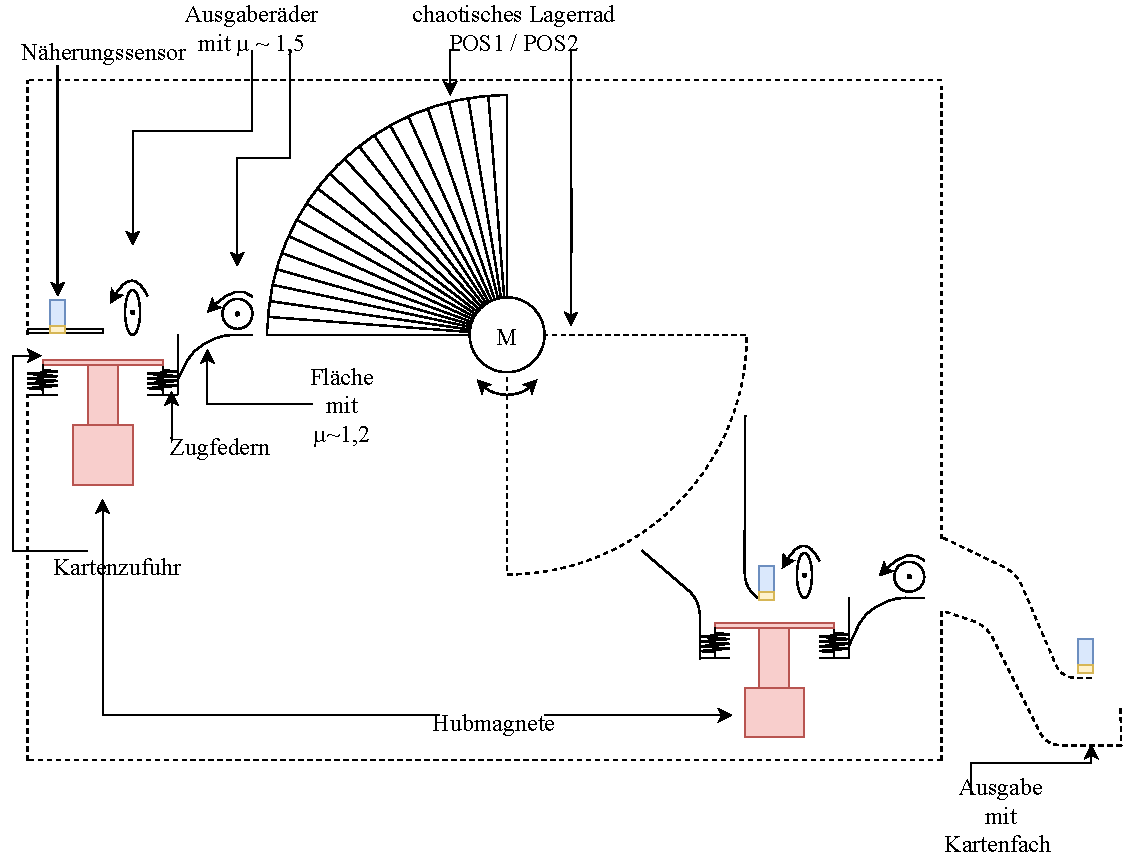
\includegraphics[width=0.6\textwidth]{fig/mech/Version2}
    \caption{Konzept 1}
\end{wrapfigure}

Beim zweiten Konzept wird als Lager ein virtel eines Zylinders benutzt. In diesem befinden
sich verschidene Fächer in der die Karten eingelagert werden. Dieser wird mit einem Motor betrieben
und dreht sich somit in die vorgegebenen Positionen um das Einlagern und das Ausgeben der Karten zu ermöglichen.
Die Karteneingabe erfolgt über einen Schlitz in der Frontplatte der Maschine, dort befindet sich ein Hubmagnet der die Karten
zum weiterbefördern nach oben drückt. Ein Kapazitiver Sensor sorgt dafür, das scihergestellt werden kann, dass sich Karten auf dem Hubmagnet befinden.
Um eine Karte in das Lager zu befördern wird der Hubmagnet eingeschaltet und drückt das Kartendeck auf das erste Ausgaberad, um die Kraft des Hubmagnetes zu minimieren sind Zugfedern angebracht.
Das Ausgaberad befördert eine Karte weiter vor zum zweiten Ausgabrad welches weiderum sicherstellt das nur eine Karten in das Lagerrad transportiert wird.
Danach dreht das Lagerrad auf eine andere zufällig ausgewählte Position. Dieser Prozess wird solange wiederholt bis alle Karten des Kartendecks sich im Lagerrad befinden.
Befinden sich alle Karten im Lagerrad, so dreht sich dieses mit einer hochen Geschwindigkeit und wirft somit die Karten auf der Hinterseite der Maschine in eine Auffangführung. %Ist Geschwindigkeit der richtige Begriff? Eher Moment oder Drehzahl?
Diese Auffangsführung befördert die Karten in einen gleichen Mechanismus wie bei der Vorderseite der Maschine, in der sie von einem Hubmagenten nach oben gedrückt werden und von zwei Ausgaberädern zur
Kartenentnahme geschoben werden. Da die Karten zum Schluss nach einem Spielmodus und somit in einer bestimmten Anzahl Ausgegeben werden, befindet sich ein Kapazitiver Sensor auch bei der Ausgabe der Karten,
dieser soll überprüfen ob die Karten von dem Spiler berreits genommen wurden oder nicht.\\

Durch den niedrigen Aufbau der durch ein "Fließbandartiges" befördern der Karten erreicht wird, besitzt die Maschine ein hohes Maß an stabilität, jedoch ensteht dadurch auch der Nachteil
dass die Maschine sehr lang wird. Da dieses Konzept 5 bewegliche Räder besitzt sowie zwei Hubmagneten ist es anfällig für Fehler beim Bewegungsablauf. Auch kann nicht garantiert werden
dass nur eine Karte in das Lagerrad befördert wird, dies würd das Konzept des optimalen Mischens zerstören. Die vielen Bauteile führen auch zu teureren Anschaffungskosten, die wir stark vermeiden möchten.\\

\textbf{Vorteile:}
\begin{itemize}
    \item stabil
    \item niedriger Aufbau
\end{itemize}
\textbf{Nachteile:}
\begin{itemize}
    \item lange Gesamtgröße
    \item viele bewegliche Bauteile / Fehlerquellen
\end{itemize}

\subsubsection{Variante 3 - Lagerrad mit Saugnäpfe}

\begin{wrapfigure}{r}{0.6\textwidth}
    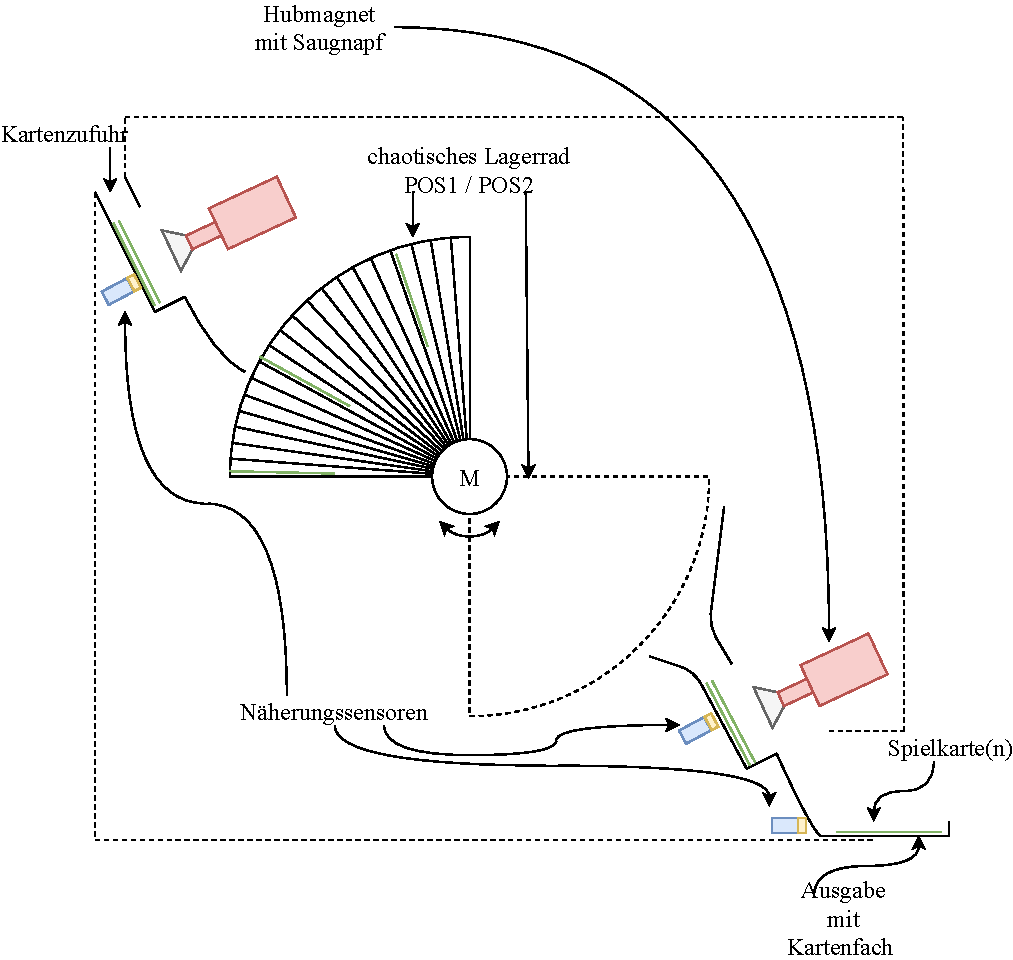
\includegraphics[width=0.6\textwidth]{fig/mech/Version3.pdf}
    \caption{Konzept 1}
\end{wrapfigure}

Das dritte Konzept besitzt ein identes Lagersystem wie das zweite Konzept, ein Lagerrad das in Fächer unterteilt ist und über einen Moter diverse Positionen einnehmen kann.
Das Kartendeck wird in den oberen / vorderen Anfang der Maschine eingeführt. Dort liegt es schräg in einem Winkel von ca. 60°. Um sicherzustellen das sich Karten in dieser Halterung befinden
ist ein Kapazitiver Sensor an der Unterseite angebracht. Ein Hubmagnet der im rechten Winkel zu den Karten über der Halterng angebracht ist, saugt jede Karte einzeln an indem ein Saugnapf der an einem Hubmagneten
befestigt ist heruntergedrückt wird. Ist die Karte angesaugt, so wird der Hubmagnet von einer Feder in seine Ausgangsstellung zurückgebracht, dabei wird die Spielkarte durch eine Platte abgestreift und fliegt somit in das Lager des
Lagerrades hinein. Dieser Prozess wird solange wiederholt bis sich alle Spilkarten des Kartendecks im Lagerrad befinden. Sind alle Karten im Lagerrad so dreht sich dieses und wirft die Karten auf der Rückseite der Maschine in ein Führung
die die Karten in eine zweite Halterung befördern. Diese zweite Halterung ist ident Aufgebaut wie die erste. Die Karten werden nun wieder einzeln vom Saugnapf angesaugt und in ein Ausgabefach am Ende der Maschine befördert. Im Ausgabefach befindet sich
ein Kapazitiver Sensor, dieser überprüft ob die Karten vom Spiler berreits genommen wurden oder nicht.\\

Durch die wenigen Bauteile die dieses Konzept besitzt, nämlich zwei Hubmagnete und einen Motor, ist das Konzept sehr fehlerunanfällig bei Bewegungsabläufe. Außerdem ist es
durch die wenigen Bauteile im vergleich billiger als die anderen Konzepte. Ein Problem dieses Konzeptes ist seine Höhe und dass das Lagerrad sich in der Mitte der Maschine befindet,
jedoch ist durch das geringe Gewicht des Lagerrades noch immer genügend stabilität vorhanden, auch wenn sich dieses mit voller Geschwindigkeit dreht. \\

\textbf{Vorteile:}
\begin{itemize}
    \item billig
    \item wenig bewegliche Bauteile
\end{itemize}
\textbf{Nachteile:}
\begin{itemize}
    \item hocher Aufbau
\end{itemize}

 \subsubsection{Ausgaberäder}
Um die Karten weiterzubefödern werden bei zwei Konzepten Ausgaberäder benutzt, für diese gibt es verschiedene Konzepte dies sich in Preis, Herstellung und Funktionalität unterscheiden.\\
Das Ausgaberad ist mit einem Motor verbunden, dieses sorgt dafür das eine Karte von einem Kartendeck weiterbefördert wird.
\begin{itemize}
    \item \textbf{Rundes Ausgaberad}
\end{itemize}
    \begin{wrapfigure}{r}{0.6\textwidth}
              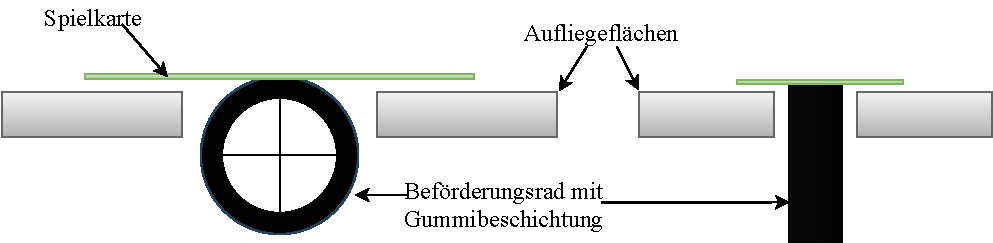
\includegraphics[width=0.6\textwidth]{fig/mech/RundesAusgaberad-Page-1}
              \caption{Konzept 1}
    \end{wrapfigure}

    Die einfachste Möglichkeit dieses Rad zu entwerfen, wäre ein einfaches rundes Ausgaberad. Dieses Rad wäre mit einer Schicht umhüllt, welche die Reibung
        dem Rad und der Karte erhöht. Das runde Rad wäre einfach zu fertigen und würde somit wenig kosten und nur einen geringen Zeitaufwand haben. Jedoch
        ist das Rad in der Lage mehr als nur eine Karte mit sich mitzuziehen, da es durchgehen Kontakt mit der Spielkartenoberfläche hat, dies hätte zur
        Folge, das mehrere Spielkarten zugleich weiterbefördert werden.
\begin{itemize}
    \item \textbf{Eliptisches Ausgaberad}
\end{itemize}
    \begin{wrapfigure}{r}{0.6\textwidth}
        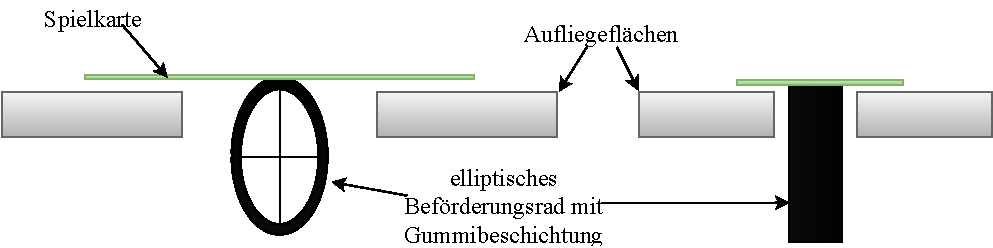
\includegraphics[width=0.6\textwidth]{fig/mech/ElliptischesAusgaberad}
        \caption{Konzept 1}
    \end{wrapfigure}

        Ein elliptisches Ausgaberad wäre das nächste Konzept, dieses Rad wird auch wie beim ersten Rad mit einem Motor verbunden um somit Karten zu befördern.
        Durch die elliptische Form des Rades herrscht kein durchgehender Kontakt mit der Oberfläche der Spilkarte, aus diesem Grund ist die Chance das mehrere
        Karten zugleich befördert werden minimiert. Jedoch setzt dies auch einen Motor vorraus der in kurzer Zeit ein hohes Drehmoment entwickelt, da die
        Karten schlagartig befördert werden. Das elliptische Rad würde in der Produktion auch mehr Kosten verursachen und wäre Zeitintesiver in der Hertellung. \\

\begin{itemize}
    \item \textbf{Vergleich der Ausgaberäder}
\end{itemize}

Da das primäre Zeil unserer Arbeit das perfekte mischen der Spielkarten ist, wäre es besser das elliptische Ausgaberad in betracht zu ziehen. Die Kosten
 die durch die aufwendigere Herstellung entstehen wären überschaulich und somit wäre es nur profitabel dieses Konzept zu wählen. Durch die Tatsache das das elliptische Rad
das Kartendeck nur jede halbe umdrehung berrührt und nicht konstant, muss ein Motor für die Räder einegesetzt werden der sich schnell genug dreht um eine Karte mit einer berührung
des Rades "herauszuschießen". Dies würde aber keine zusätzlichen Kosten verursachen. Aus diesen Gründen fällt die Wahl auf das \textbf{elliptisches Ausgaberad}. \\
\subsection{Klemmmechanissmen}
Um beim Ausgeben und beim Weiterbefördern der Karten die Chance zu minimieren das mehrere Karten auf einmal weiterbefördert werden, wird ein
Klemmmechanissmus benutzt, dieser sorgt dafür das die Karten von außen Geklemmt werden, und somit nur die unterste Karte durch das Drehen des
Ausgaberades weiterbefördert wird.

\begin{itemize}
    \item \textbf{primitiver Klemmmechanissmus}
\end{itemize}

\begin{wrapfigure}[12]{r}{0.6\textwidth}
    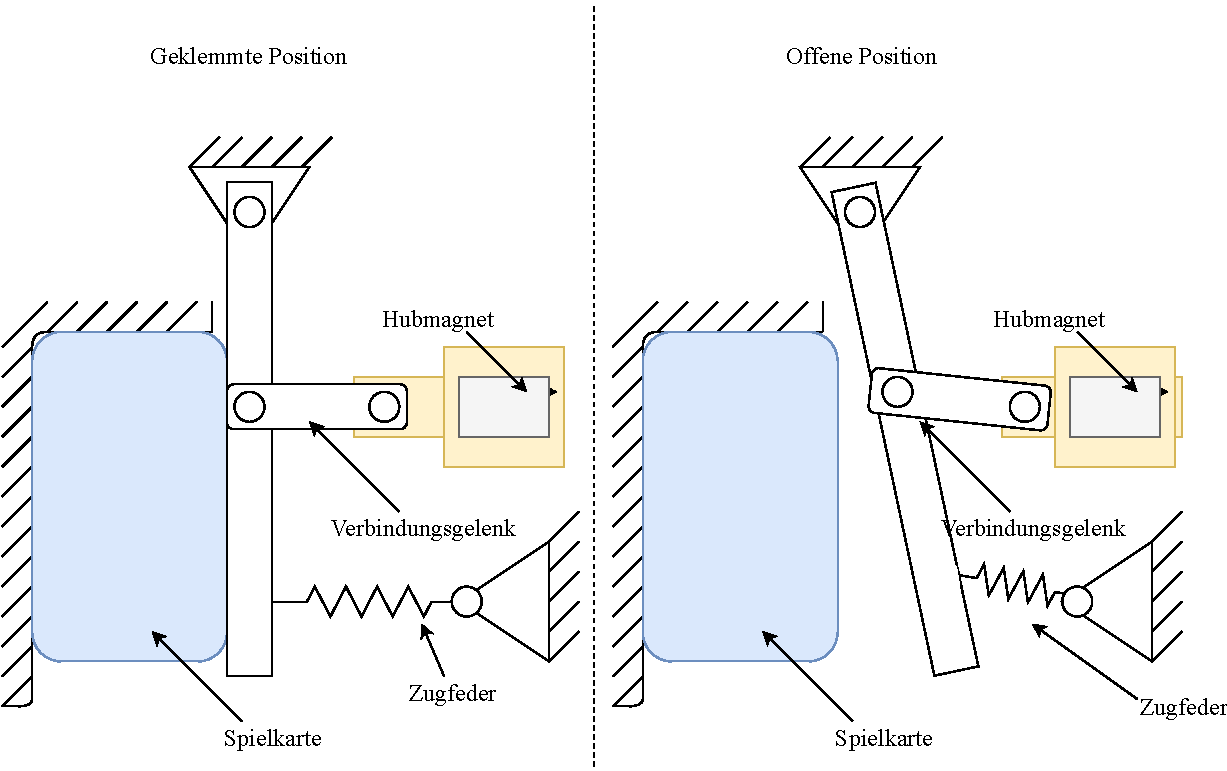
\includegraphics[width=0.6\textwidth]{fig/mech/Klemmmechanissmus1}
    \caption{Konzept 1}
\end{wrapfigure}

Dieser Klemmmechanismus ist der primitivste und einfachste, dadurch aber auch der billigste. Die Karten werden auf der einen Seite an eine feste Wand gedrückt
auf der anderen Seite werden sie durch ein bewegliches Gelenk fixiert. Dieses Gelenk wrid durch das einschalten des Hubmagneten in die geschlossene Position bewegt,
soll das Gelenk wieder öffnen, so wird der Hubmagnet ausgeschalten und ein Zugfeder zieht das Gelenk wieder in seine Ausgangsposition zurück.

\begin{itemize}
    \item \textbf{Komplexer Klemmmechanissmus}
\end{itemize}
\begin{wrapfigure}[12]{r}{0.6\textwidth}
    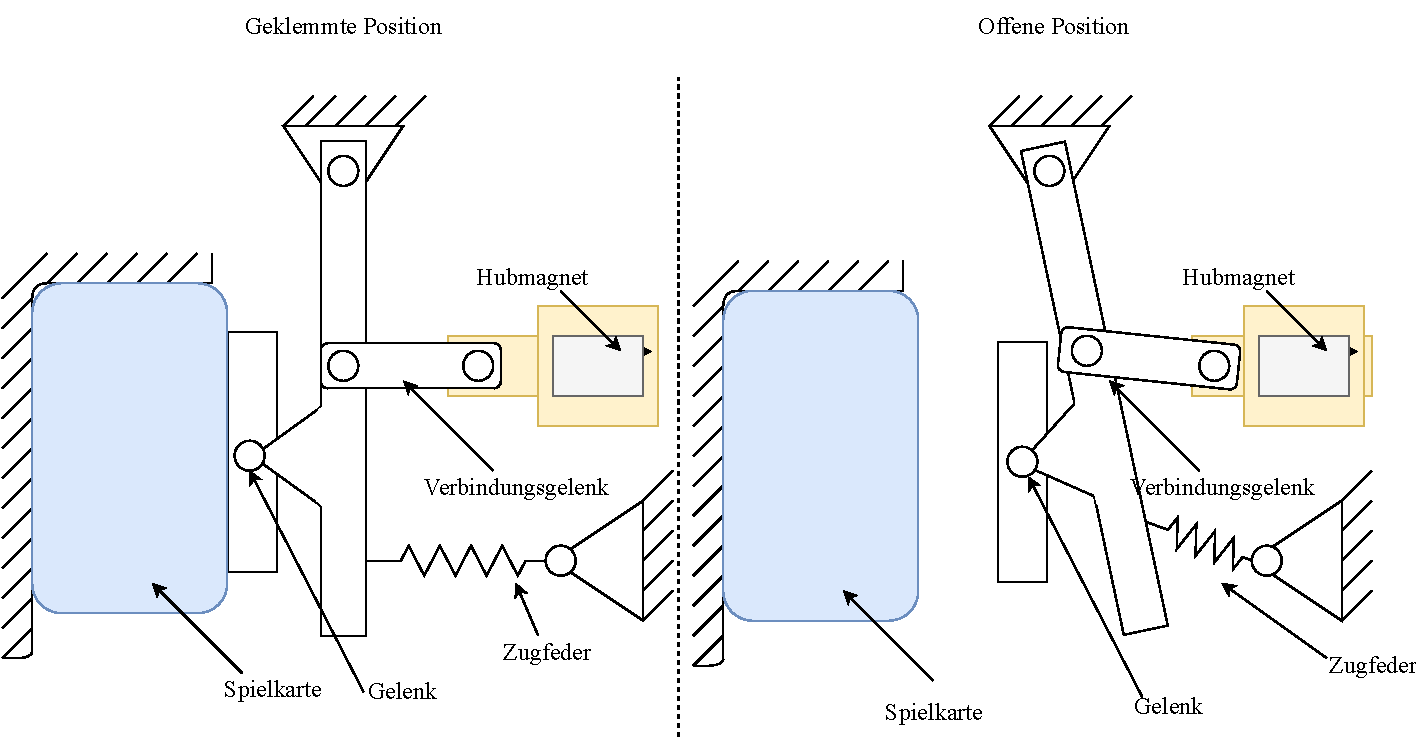
\includegraphics[width=0.6\textwidth]{fig/mech/Klemmmechanissmus2}
    \caption{Konzept 1}
\end{wrapfigure}

Bei diesem Mechanissmus werden die Karten auf der einen Seite durch eine feste Wand geklemmt, auf der anderen werden sie durch ein Gelenk geklemmt, dieses Gelenk
ist beweglich und gleicht somit verschidene Kartengrößen aus. Um das Gelenk dieses Konzeptes zu schliesen wird ein Hubmagnet benötigt, wird dieser eingeschalten
so schließt das Gelenk und passt sich der Kartengröße an. Soll es wieder geöffent werden, so wird der Hubmagnet ausgeschaltet und eine Zugfeder bringt den Mechanissmus wieder in den
Grundzustand. Dieses Konzept ist aufwendiger zu realisieren wie das erste, jedoch kann es verschiedene Kartengrößen klemmen und gleicht sich den Karten an. Das Konzept ist
dafür aber auch aufwendiger in der Produktion.

\begin{itemize}
    \item \textbf{Gummi Klemmmechanissmus}
\end{itemize}
\begin{wrapfigure}[12]{r}{0.6\textwidth}
    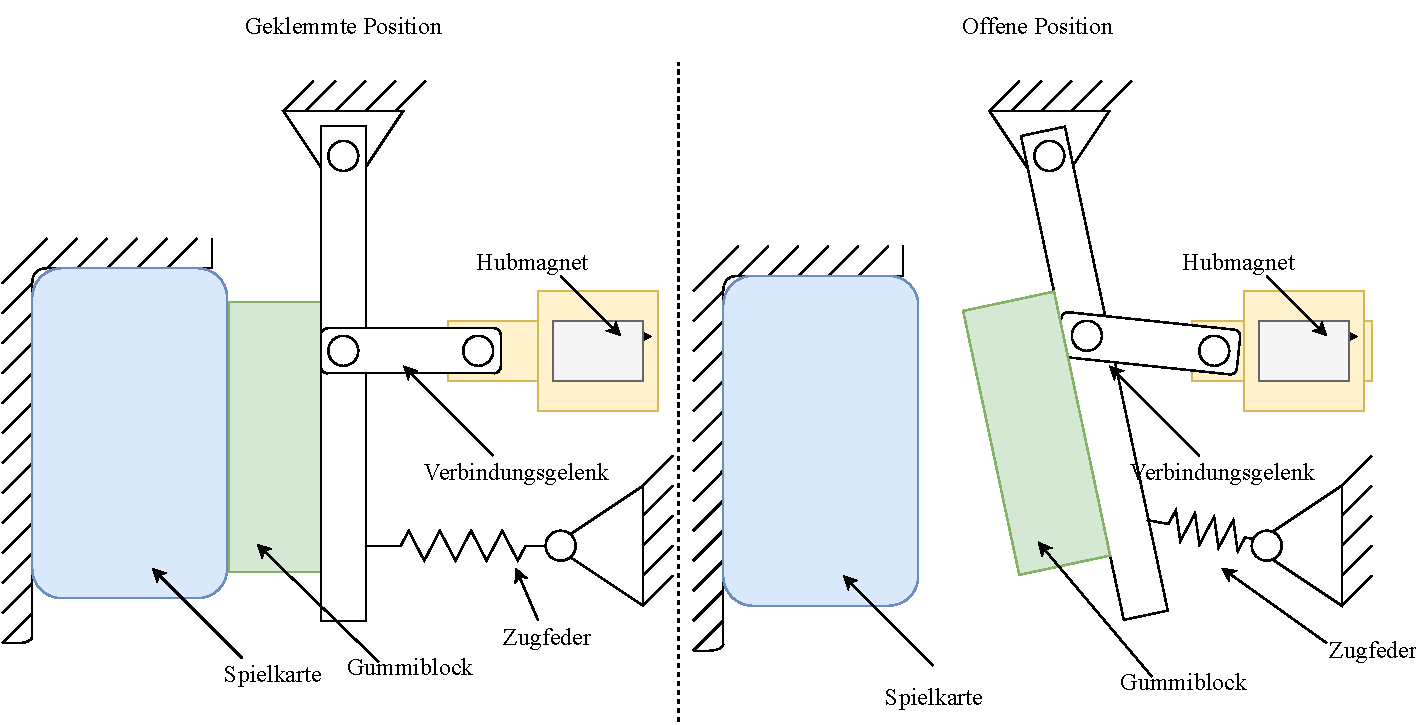
\includegraphics[width=0.6\textwidth]{fig/mech/Klemmmechanissmus3}
    \caption{Konzept 1}
\end{wrapfigure}

Der letzte Mechanissmus ist ufnktionsmäsig gleich wie der primitive Klemmmecahnissmus, der einzige Unterschied besteht aus dem
Gummiähnlichen Block der auf der Klemmfläche sitzt. Dieser soll sich den Karten anpassen und sorgt dafür das alle Karten gleichmäßig
 geklemmt werden, auch erhöht es die Reibung zwischen den Karten und der Klemmoberfläche. Dieses Konzept wäre in der  Herstellung verglichsweise
eifnach zu realisieren und dadurch auch billig in der Herstellung.


\begin{itemize}
    \item \textbf{Vergleich der Klemmmechanissmen}
\end{itemize}

Da alle Mechanissmen die gleiche Anzahl an Bateile erfordern, spielt der Pries bei dieser Auswahl keine große Rolle. Aus diesem Grund
sind die Kriterien Funktionalität und Aufwendigkeit in der Produktion. Der erst Mechanissmus wäre der einfachste in der Produktion, jedoch
hat er durch sein nicht anpassungsfähiges Klemmgelenk Probleme mit verschiedenen Kartengrößen, aus diesem Grund fällt er bei diesem Auswahlverfahren durch.
Der zweite Mechanissmus wäre der komplexe Klemmmechanissmus, dieser würde sich zwar verschiedenen Kartengrößen anpassen, wäre aber etwas aufwendiger in der
Produktion und ist somit auch nicht die bevorzugte Wahl. Der letzte Klemmechanissmus der einen gummiartigen Block auf der Klemmfläche hat, wäre einfach in der
Produktion und würde sich auch bei verschiedenen Kartengrößen anpassen, aus diesem Grund  fätt die wahl auf den Gummi Klemmmechanissmus.

\section{Konstruktion}

\section{Berechnungen, Festigkeitsanalyse und Dimensionierungen}

\section{Teilaufbau}